\subsection{Bagging}
\begin{figure}
    \centering
    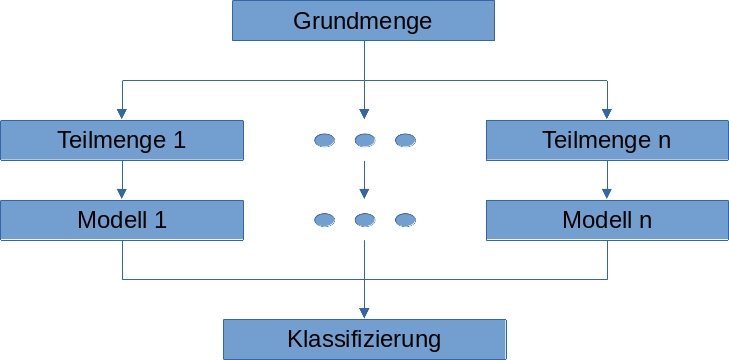
\includegraphics[width=0.6\linewidth]{images/bagging.jpg}
    \caption{Klassifizierungsprozess mit der Bagging-Methode.}
    \label{fig:bagging}
\end{figure}
Bagging ist ein Acronym für \glqq \textbf{B}ootstrap \textbf{agg}regat\textbf{ing}\grqq. Die Idee ist aus einer großen Menge von Trainingsdaten, eine Menge von Mengen von Trainingsdaten zu generieren, folgend mit jedem
dieser Mengen einen Klassifizierer zu trainieren und schließlich alle Klassifizierer, e.g. durch Wählen, zu aggregieren (siehe Abbildung \ref{fig:bagging}) \cite{breiman1996bagging}. Die Methode die dahinter steht nennt
sich \glqq Bootstrap sampling\grqq, welche einen Prozess beschreibt aus einer Grundmenge $m$ mal jeweils $n$ Einträge zu ziehen, die eine Teilmenge bilden \cite{efron1992bootstrap}. Der Name ist folglich aus der Methode
und dem Aggregierungsprozess abgleitet.